\documentclass[12pt,twoside,openright,a4paper,english,brazil,sumario=tradicional]{abntex2}
\usepackage[utf8]{inputenc}
\usepackage[T1]{fontenc}
\usepackage{indentfirst}
\usepackage{color}
\usepackage{graphicx}
\usepackage{microtype}
\usepackage[brazilian,hyperpageref]{backref}
\usepackage[alf]{abntex2cite}
\usepackage{multicol}
\usepackage{multirow}
\usepackage{enumitem}
\usepackage{amsfonts}
\usepackage{amssymb}
\usepackage{listings}
\usepackage{tikz-uml}
\usepackage{uarial}
\usepackage{blindtext}
\usepackage{float}
\usepackage{pdfpages}
\graphicspath{{../images/}}
\renewcommand{\familydefault}{\sfdefault}
\renewcommand{\backrefpagesname}{Citado na(s) página(s):~}
\renewcommand{\backref}{}
\renewcommand*{\backrefalt}[4]{
   \ifcase #1 %
   Nenhuma citação no texto.%
   \or
   Citado na página #2.%
   \else		Citado #1 vezes nas páginas #2.%
   \fi}%
\newfloat{mylisting}{tbphH}{lopbl}[chapter]
\floatname{mylisting}{Listing}
\newsubfloat{mylisting}
\newcommand{\listofmylistings}{\listof{mylisting}{List of Listings}}
% if you use the hyperref package
\providecommand*\theHmylisting{\themylisting}
\newcommand{\listbylist}[6][showlines=true]{
  \begin{mylisting}
    \subfloat[ ]{
      ...
    }
    \hfill{}
    \subfloat[ ]{
      ...
    }
    \hfill{}
    \caption[#5]{#6}
    \label{#4}
  \end{mylisting}
}
\titulo{Módulo de pré visualização para a ferramenta CGT - Ceará Game Tools}
\author{Joel Xavier Rocha\thanks{\texttt{joelxr@gmail.com}}}
\orientador{Prof. Dr. Carlos Hairon Ribeiro Gonçalves}
\local{Fortaleza}
\data{2015}
\instituicao{
   Instituto Federal de Ciência, Educação e Tecnologia do Ceará
   \par
   Engenharia de Computação}
\tipotrabalho{Monografia}
\preambulo{Trabalho de conclusão de curso apresentado à banca examinadora do Instituto Federal de Educação, Ciência e Tecnologia do Ceará para obtenção do grau de bacharel em Engenharia de Computação sob a orientação do Prof. Dr. Carlos Hairon Ribeiro Gonçalves.}
\definecolor{blue}{RGB}{41,5,195}
\makeatletter
\hypersetup{
   pdftitle={\@title},
   pdfauthor={\@author},
   pdfsubject={Trabalho de conclusão de curso},
   pdfcreator={pdfLaTeX},
   pdfkeywords={abnt}{latex}{abntex}{abntex2}{trabalho científico},
   colorlinks=true,
   linkcolor=blue,
   citecolor=blue,
   filecolor=magenta,
   urlcolor=blue,
   bookmarksdepth=4
}
\makeatother
\setlength{\parindent}{1.3cm}
\setlength{\parskip}{0.2cm}
\makeindex
\begin{document}
\lstset{
        frame=single,
        showlines=true,
        language=java,
        tabsize=3,
        basicstyle=\scriptsize
        }
\selectlanguage{brazil}
\frenchspacing
\imprimircapa
\imprimirfolhaderosto*

% \begin{fichacatalografica}
%     \includepdf{fig_ficha_catalografica.pdf}
% \end{fichacatalografica}

% \includepdf{folhadeaprovacao_final.pdf}

\begin{agradecimentos}

\end{agradecimentos}
\setlength{\absparsep}{18pt}
\begin{resumo}
   O crescimento da industria de jogos em diversas áreas - como entretenimento e educação - torna necessário a elaboração de ferramentas que possibilitem a criação destes de forma simples, fácil e objetiva. Por esta razão, o projeto \emph{Ceará Game Tools} (CGT), tem como objetivo possibilitar isso aos usuários que não conhecem os meios e as técnicas envolvidas na criação de jogos.

   Então, é proposto nesse trabalho, melhorias importantes para a ferramenta CGT, principalmente, a pré visualização do jogo que está sendo construído e também dos seus objetos.

   \vspace{\onelineskip}
   \noindent
   \textbf{Palavras-chave}: CGT, ferramenta;
\end{resumo}
\pdfbookmark[0]{\listfigurename}{lof}
\listoffigures*
\cleardoublepage
\pdfbookmark[0]{\listtablename}{lot}
\listoftables*
\cleardoublepage
\pdfbookmark[0]{\contentsname}{toc}
\tableofcontents*
\cleardoublepage
\textual
\chapter{Introdução} % Ryllari
\label{chap:introducao}
% introduzindo sobre o que é o trabalho
Neste trabalho, é apresentado problemas existentes e pontos de melhorias na primeira versão da ferramenta de construção de jogos do projeto CGT (\texttt{ferramenta 1.0}). Bem como, de que modo essas questões foram tratadas e implementadas na segunda versão (\texttt{ferramenta 2.0}). A nova versão da ferramenta tem como objetivo melhorar o processo de criação de jogos e tornando-o mais intuitivo para o usuário final.
\section{O projeto CGT}
% Descrição/apresentação do projeto CGT
O projeto CGT que surgiu para tornar possível a qualquer pessoa a criação de jogos, assim como é explicado no trabalho \cite{monografia:aquino}, vem sido desenvolvido desde 2013 e possibilita a construção de jogos eletrônicos por qualquer pessoa, não sendo necessário conhecimentos em programação ou nas técnicas de criação de jogos. De foma fácil, simples e prática, a ferramenta, atende a necessidade da maior parte dos usuários, podendo produzir jogos de vários temas e para diversos fins, desde entretenimento a educação, por exemplo. Assim como, é proposto no \emph{website} do projeto que explica, detalhadamente, o seu objetivo.
\begin{citacao}
   O projeto Ceará Game Tools tem como objetivo oferecer uma ferramenta para a construção de jogos. Em suma, qualquer um poderá criar seu próprio jogo utilizando componentes \emph{drag and drop} e os configurando. \cite{website:projeto-cgt}
\end{citacao}
\subsection{Vínculo com o CNPQ}
A idealização e o início do desenvolvimento da ferramenta CGT deu-se no ano de 2013, através do projeto Ceará Game Tools (CGT) – Pesquisa, Desenvolvimento e Comercialização de Games Temáticos da Cultura Cearense, que é uma inciativa do professor do IFCE Carlos Hairon Ribeiro Gonçalves  apoiado pelo CNPQ\footnote{Centro Nacional de desenvolvimento científico e tecnológico.} por meio do edital 80 de 2013 de número de processo 409227/2013-7.

A proposta deste projeto era desenvolver uma ferramenta de software livre para o desenvolvimento automático de \emph{games} casuais em que qualquer pessoa com conhecimentos medianos de operação de microcomputadores poderia desenvolver jogos. Neste caso, não há necessidade de codificação de software utilizando-se linguagens de programação, mas somente o desenvolvimento de modelos abstratos com o uso de aplicativos de software de uso livre. Além disso, ela pode gerar jogos que podem ser executados em vários sistemas operacionais(\emph{Windows}, \emph{Linux}, \emph{MacOS} e \emph{Android}). Desse modo, os desenvolvedores podem aferir retorno financeiro com a venda e/ou popularização dos jogos, democratizando este canal para todas as pessoas que queiram ingressar nessa área.
\subsection{Trabalhos anteriores}
A partir do projeto vinculado ao CNPQ, a primeira versão da ferramenta foi produzida, trabalhando o desenvolvimento dos jogos apenas com entrada e manipulação de dados, utilizando apenas botões e comandos, sem componentes \emph{drag and drop} ou módulo de pré-visualização. Com base no que foi desenvolvido ao longo desta etapa, foi produzido um trabalho acadêmico de conclusão de curso por título “Ceará Game Tools: Uma ferramenta de software livre para geração automática de games” \cite{monografia:aquino}.

Em aspectos gerais, esse trabalho apresenta todo o processo de criação da ferramenta Ceará Game Tools (CGT), que possui um ambiente de desenvolvimento visual simples e intuitivo e uma biblioteca de imagens e sons disponibilizados para os usuários desfrutarem. Além disso, nesse trabalho, relata trabalhos e \emph{softwares} similares ao CGT, descreve os métodos e ferramentas utilizados para o desenvolvimento da aplicação, além da forma com ela foi desenvolvida, os módulos em que o CGT está dividido, os pacotes e classes que compõem a ferramenta, seus diagramas, benefícios, bem como trabalhos futuros e possíveis melhorias para a ferramenta. Nesta última parte, o autor destaca a importância da criação de novas políticas que aumentem as opções dos jogos e implementem novas estruturas, do aumento no número de plataformas de exportação dos jogos desenvolvidos, além de adicionar módulo de pré-visualização do jogo, o qual se concentra o assunto do presente trabalho.

\subsection{Os módulos desenvolvidos para o projeto}
% ferramenta de construção de jogos
O projeto é composto por módulos que dividem as funcionalidades existentes, esses módulos são mostrados e descritos na tabela \ref{table:modulos}. O módulo da ferramenta que é o objeto de estudo para este trabalho tem como objetivo implementar toda a interação com o usuário e ser responsável por apresentá-lo ao jogo no momento da criação, tudo isso de forma intuitiva, simples e prática. Pode-se notar que, esse módulo é essencial para o projeto e deve ser capaz de lidar com tudo que torna possível a criação de jogos.
\begin{table}[h]
   \centering
   \begin{tabular}{ | l | p{10cm} | }
      \hline
      \textbf{Módulos} & \textbf{Descrição} \\
      \hline
      \texttt{core} & Contém os objetos essenciais para o projeto. Assim como: Ator, Inimigo, Bônus. Na secção \ref{sec:objetos} pode ser visto todos os objetos. \\
      \hline
      \texttt{desktop} & Responsável por possibilitar a execução do jogo no computador, em ambientes que rodam os sistemas \emph{Windows}, \emph{Linux} e \emph{MacOS}. \\
      \hline
      \texttt{ferramenta} & Corresponde ao módulo objeto de estudo deste trabalho que possibilita a criação dos jogos. \\
      \hline
      \texttt{android} & Permite exportar o jogo para execução nos dispositivos que rodam o sistema operacional \emph{Android}. \\
      \hline
      \texttt{ios} & Permite exportar o jogo para execução nos dispositivos que rodam o sistema operacional \emph{iOS}. \\
      \hline
   \end{tabular}
   \caption{Módulos existentes no projeto CGT.}
   \label{table:modulos}
\end{table}
\section{Introdução ao problema}
\label{sec:intro-problema}
A identificação dos problemas e pontos de melhoria para a ferramenta foram percebidos, principalmente, através do uso e estão relacionados a interação com o usuário final, além disso, na forma como o jogo em produção é percebido.

A \texttt{ferramenta 1.0} é bastante robusta e atende o propósito de criar os objetos que compõem o jogo e, eventualmente, produzi-lo em forma de aplicação para a plataforma destino. Entretanto, a mesma carece em fornecer algum \emph{feedback} no momento da criação, obrigando ao usuário a sempre executar o jogo para poder perceber atributos essenciais dos objetos dele, tais como: a posição, o tamanho, a textura.

Por exemplo, sejam as posições de um novo objeto configuradas da forma que se deseja, logo após isso, naturalmente, o usuário executa o jogo para poder visualizar o que configurou, e também entender o que representa graficamente o número que inseriu. Pode-se ver esse processo ocorrendo na imagem \ref{fig:intro-problema-1}, as duas janelas que estão abertas são, respectivamente, a do jogo em execução e da ferramenta de criação. Portanto, podemos assumir que para todo objeto recém configurado, será preciso executar o jogo para ver o resultado da configuração, ou seja, o processo de criação se torna bastante repetitivo.

\begin{figure}[h]
   \centering
   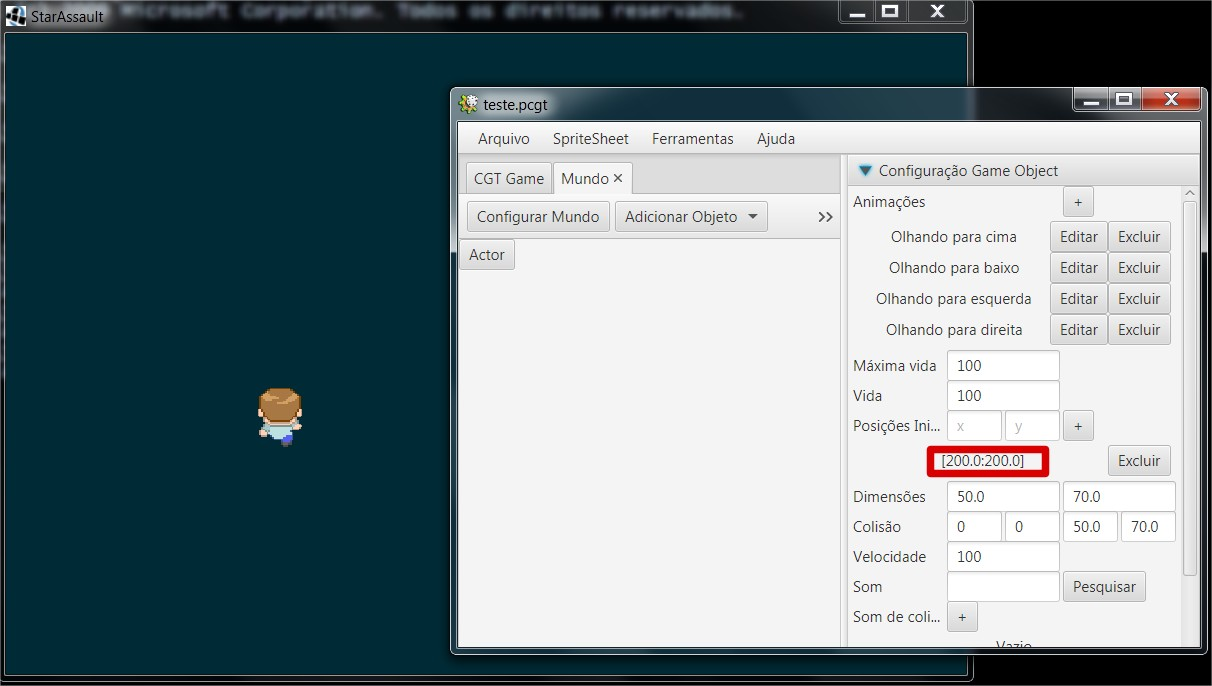
\includegraphics[width=0.7\textwidth]{images/problema-1.jpg}
   \caption{Problema de pré-visualização na \texttt{ferramenta 1.0}.}
   \label{fig:intro-problema-1}
\end{figure}

% mais problemas
Além disso, os controles que fazem parte da primeira versão da ferramenta, tornam, na maioria das vezes, oneroso o processo de configuração dos objetos. Por exemplo, na configuração das animações que possui um objeto é necessário criar as animações olhando no \emph{spritesheet}\footnote{Imagem que contém todas as faces de um objeto no jogo.} do objeto e preenchendo campos de texto com o valor da linha e coluna do \emph{sprite} correspondente a animação configurada (ver imagem \ref{fig:intro-problema-2}).

\begin{figure}[h]
   \centering
   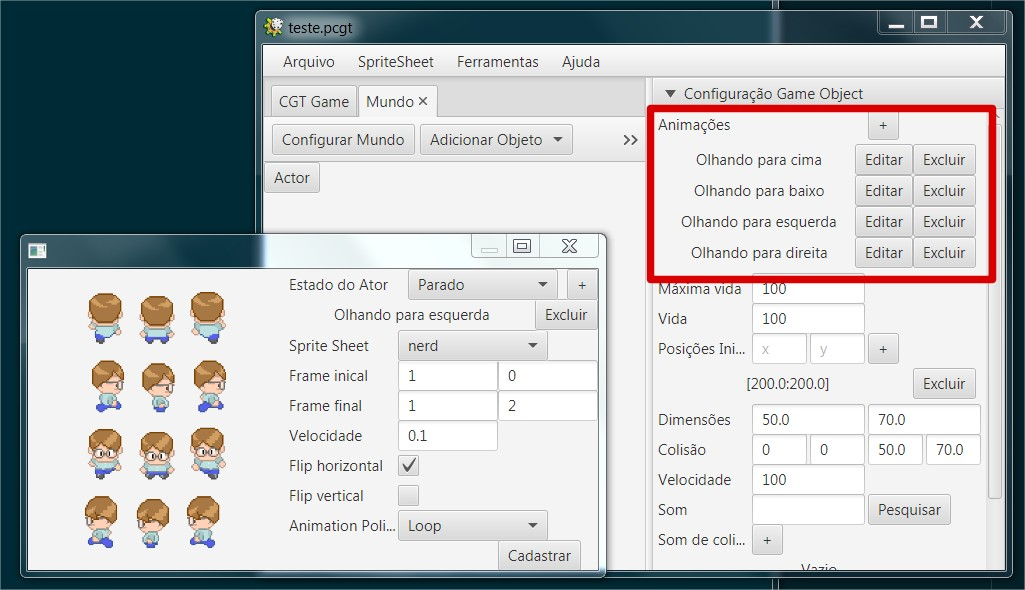
\includegraphics[width=0.7\textwidth]{images/problema-2.jpg}
   \caption{Problema com os controles na configuração de uma animação na \texttt{ferramenta 1.0}.}
   \label{fig:intro-problema-2}
\end{figure}

Os problemas encontrados na \texttt{ferramenta 1.0} foram a motivação para esse trabalho e serão descritos detalhadamente no capitulo \ref{chap:problemas}.

\section{Disposição do documento}
Este documento segue o método que consiste em: apresentar um problema, propor sua solução e, por fim, estudar as consequências da solução adotada. Dessa forma, tudo estará dividido basicamente nas três partes seguintes:
\begin{description}
   \item[Definição do problema] Mostrado no capítulo \ref{chap:problemas} que tem como objetivo enumerar detalhadamente os problemas e pontos de melhoria encontrados na \texttt{ferramenta 1.0} e como foram encontrados. Consequentemente, prepara-se uma lista das principais funcionalidades que farão parte da nova versão da ferramenta.
   \item[Proposta de melhorias] Corresponde ao capítulo \ref{chap:melhorias} que visa propor soluções para as questões encontradas anteriormente. Além disso, explicá-las e justificá-las detalhadamente, por fim demonstrando a solução adotada e como elas foram alcançadas.
   \item[Análise dos resultados] É um estudo de caso, mostrado no capítulo \ref{chap:caso}, com a nova versão da ferramenta, onde busca-se comparar o tempo de criação de jogo, a facilidade de uso e a quantidade de esforço necessário para configurar.
\end{description}

\chapter{Problema}
\label{chap:problemas}
% breve descrição do problema do preview
A ferramenta de construção de jogos do projeto CGT é robusta e atende aos objetivos propostos. Contudo, ela possui lacunas quando se trata da interação humano computador (IHC). A falta de pré-visualização dos objetos contidos no jogo dificulta a percepção do usuário, obrigando-o a sempre executar o jogo para observar as configurações que foram feitas. Além disso, os controles não são claros e, assim, produzir um jogo pode acabar sendo uma experiência onerosa, confusa e repleta de configurações repetitivas.

A nova versão da ferramenta visa resolver os dois problemas mencionados, principalmente o primeiro item, por ser mais importante quando o assunto é usabilidade. Com isso em mente, faz-se necessário construir um jogo na primeira versão da ferramenta com o objetivo de perceber os problemas e as possíveis melhorias.

\section{Objetos de um jogo}
\label{sec:objetos}

Para enumerar todos os problemas e melhorias da \texttt{ferramenta 1.0}, é importante construir um jogo com ela, então é preciso conhecer os objetos que existem nele e como eles são configurados. Observar que, cada um deles possui suas características e configurações, assim como um propósito no jogo, a tabela \ref{table:objetos-desc} mostra os possíveis tipos objetos e a descrição deles. Notar que, eles são inseridos na ferramenta a medida que o usuário ver necessidade e são responsáveis por dar liberdade ao autor de construir vários formatos de jogos, por exemplo jogos de: perguntas e respostas, concluir percurso, derrotar inimigo, sobreviver determinado tempo.

\begin{table}[htb]
\centering
\begin{tabular}{| l | p{7cm} |}
      \hline
      \textbf{Objeto} & \textbf{Descrição} \\
      \hline
      Mundo & Responsável por agregar todos os personagens de uma fase do jogo definindo o plano de fundo.  \\
      \hline
      Ator & Objeto controlado pelo jogador. \\
      \hline
      Inimigo & Objeto que causa dano ao ator e impede os objetivos dele. \\
      \hline
      Opositor & Objeto que impede ações do ator, que não pode ser ultrapassado e pode ser destruído pelo ator.  \\
      \hline
      Bônus & Objeto que promove bônus ao ator. \\
      \hline
      Projétil & Objeto que pode ser arremessado pelo ator. \\
      \hline
      Tela & Representa uma tela do jogo. \\
      \hline
      Botão de tela & Botão de uma tela do jogo. \\
      \hline
      Vida de um objeto & Representado através de uma barra, mostra a quantidade de vida que um objeto possui. \\
      \hline
      Munição de um objeto & A quantidade de projéteis que o ator ainda pode arremessar. \\
      \hline
   \end{tabular}
\caption{Objetos que existem em um jogo.}
\label{table:objetos-desc}
\end{table}

A seguir, pode ser visto um jogo de exemplo na ferramenta e, com isso, os problemas e pontos de melhoria. O manual da ferramenta está nos anexos para ser consultado com o objetivo de entender como funciona a criação de cada um desses objetos.

\section{Dificuldades encontradas}
\label{sec:dificuldades}
A medida que a ferramenta foi utilizada, achou-se dificuldades que podem ser qualquer interação confusa com a ferramenta ou que dificulta a criação e configuração de algum objeto, assim como o entendimento do papel dele no jogo. Essas dificuldades, embora pareçam subjetivas, podem ser mensuradas e quantificadas normalmente. As demais seções desde capítulo, encarregam-se de trazer esses problemas, dentre eles existe, por exemplo, a dificuldade de observar um objeto, após alterar alguma propriedade dele.
Notar que, a \texttt{ferramenta 1.0} está disponível no \href{http://www.cgt.ifce.edu.br/downloads.php}{site do projeto CGT} na secção de \emph{downloads}\footnote{http://www.cgt.ifce.edu.br/downloads.php}.

\subsection{Organização dos objetos}
\label{sec:orga-objetos}
Um dos pontos mais importantes quando se trata de criação de jogos, é que - no decorrer do desenvolvimento - eles podem se tornar enormes e, para a ferramenta, um jogo é um conjunto de objetos e suas respectivas propriedades. Logo, é imprescindível que os objetos possam ser vistos de forma lógica e, mais importante, organizada, já que, assim, serão acessados facilmente, pois o usuário terá necessidade de retornar a eles para melhorar ou corrigir alguma configuração. Além disso, vale ressaltar que entre os objetos existe uma relação de pertinência, um ator está inserido em um mundo, assim como o inimigo que ele precisa derrotar também o está, essa hierarquia precisa ser levada em consideração na ferramenta e o jogo será criado respeitando essas relações.

Na figura \ref{fig:objetos_disp}, pode-se visualizar um jogo sendo criado e - a partir dessa imagem - pode-se notar que a ferramenta é dividida em cinco áreas importantes (descritas na tabela \ref{table:ferramenta_areas}). Os botões que representam objetos são organizados por colunas que representam as categorias: ator, inimigos, opositores, bonificações e informações da tela. A medida que é adicionado um novo objeto para a aba, este é posicionado em uma dessas colunas. Essa forma de organizar os objetos do jogo, possui a vantagem de ser objetiva, pois exibe apenas o conteúdo que importa para aquele agregador (uma fase do jogo ou uma tela). No entanto, a medida que o usuário vai inserindo elementos ao jogo e configurando eles, essa visão pode perder o significado, isto é, precisa-se de algo além de um botão com um nome gerado automaticamente para representar um objeto e ser identificado facilmente pelo usuário. Como pode ser visto na figura \ref{fig:objetos_disp}, nesse jogo, existem quatro inimigos configurados, mas não se sabe quais são as características deles apenas olhando para os botões, ou seja, o usuário precisa selecionar um a um até encontrar qual deles é o que ele procura, qual deles é o inimigo final da fase, por exemplo. Sendo assim, a ação de reconfigurar um objeto pode tornar-se difícil a medida que novos itens forem sendo adicionados ao jogo.

\begin{table}[h]
   \centering
   \begin{tabular}{| l | p{8cm} |}
      \hline
      \textbf{Menu} & No menu é possível realizar ações que refletem no projeto todo, por exemplo: salvar, adicionar \emph{spritesheet}, executar o jogo. \\
      \hline
      \textbf{Abas} & As abas representam os agregadores de objetos, podem conter a aba inicial do projeto, um \emph{mundo} ou uma tela. \\
      \hline
      \textbf{\emph{Toolbar}} & Permite realizar ações referentes ao agregador, se for de um mundo possibilitar adicionar um inimigo ao jogo, por exemplo. \\
      \hline
      \textbf{Botões de objetos} & Cada objeto é representado por um botão que pertencem a uma determinada aba. \\
      \hline
      \textbf{Painel lateral} & Mostra as configurações do objeto selecionado, ao clicar em qualquer botão será mostrado as configurações daquele objeto.  \\
      \hline
   \end{tabular}
   \caption{Controles utilizados na primeira versão da ferramenta.}
   \label{table:ferramenta_areas}
\end{table}

\begin{figure}[h]
\centering
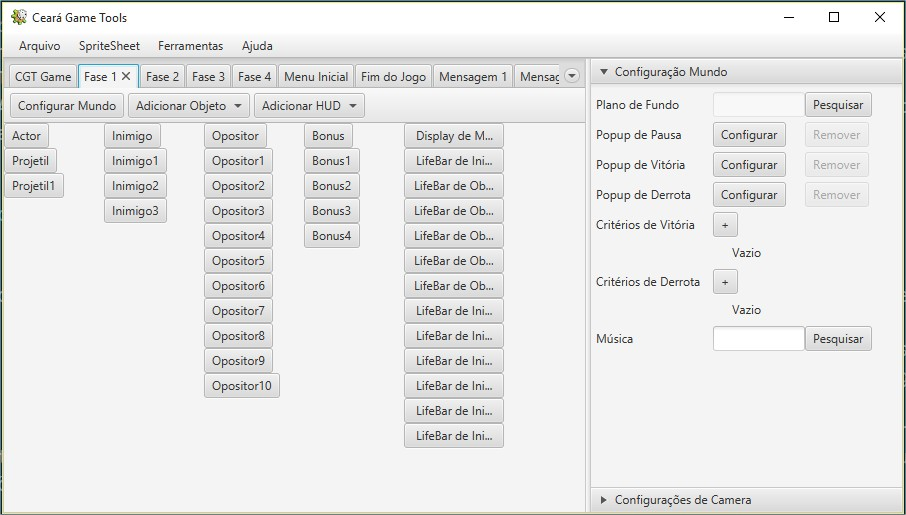
\includegraphics[width=0.8\textwidth]{images/objetos_disposicao.jpg}
\caption{Disposição dos objetos na versão anterior da ferramenta.}
\label{fig:objetos_disp}
\end{figure}

\subsection{Painéis de configuração dos objetos}
\label{sec:paineis-objetos}
Todos os itens que fazem parte de um jogo possuem características que os definem, sendo assim cabe a ferramenta prover ao usuário final uma forma clara e objetiva de configurá-las. Além disso, a ferramenta tem obrigação de validar os dados e guiar o usuário nos casos mais complexos, assim como dar um significado para o dado que está sendo recebido. Por exemplo, vamos supor que exista um objeto recém adicionado no jogo e que pretendemos configurar a sua posição inicial na tela, a ferramenta recebe essa configuração através de dois números que são, respectivamente, as posições cartesianas $x$ e $y$ do objeto, deve-se verificar se essas posições estão contidas no retângulo que representa a tela do jogo, assim como fornecer ao usuário formas de saber o que significa o valor que ele está configurando. Essa e outras propriedades possuem a mesma necessidade de serem visualizadas, ver tabela \ref{table:objetos-atributos}.

\begin{figure}[h]
\centering
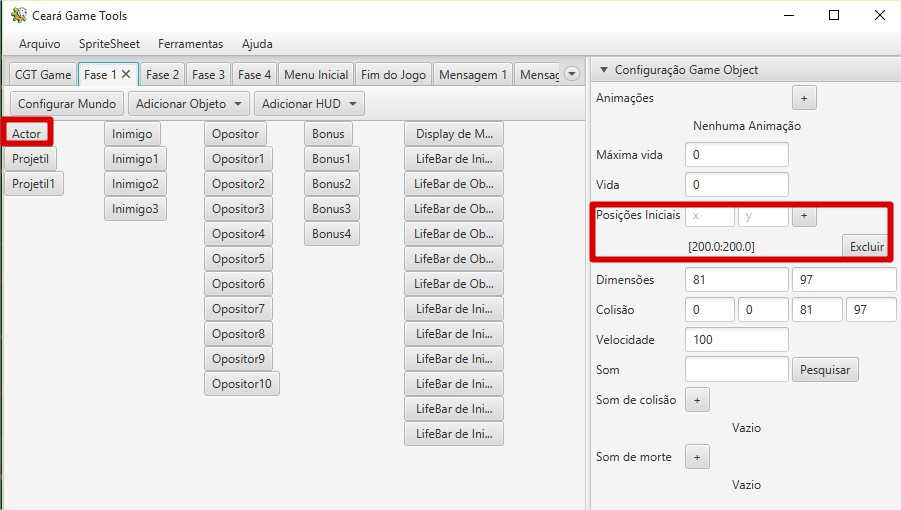
\includegraphics[width=0.8\textwidth]{images/pos_inicial.jpg}
\caption{Configuração da posição inicial de um objeto na primeira versão da ferramenta.}
\label{fig:obj_pos_inicial}
\end{figure}

\begin{figure}[h]
\centering
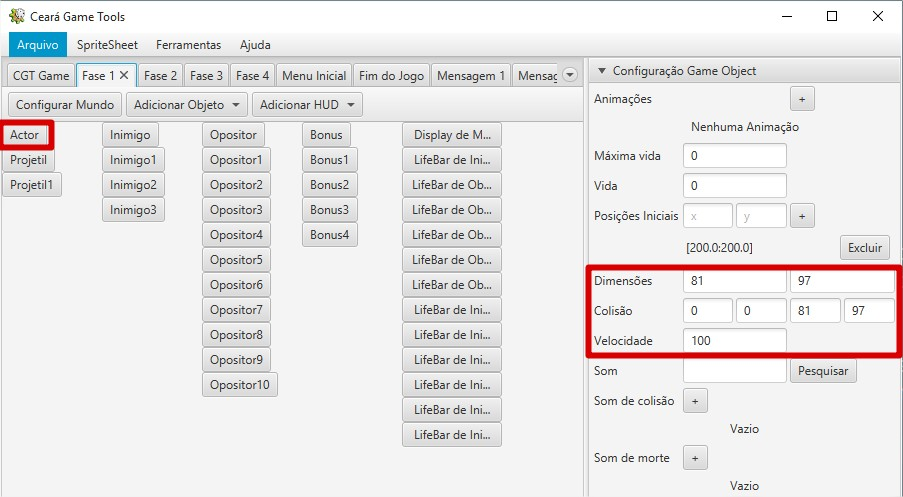
\includegraphics[width=0.8\textwidth]{images/obj_dimensoes.jpg}
\caption{Configuração das dimensões de um objeto na primeira versão da ferramenta.}
\label{fig:obj_dimensoes}
\end{figure}

\subsection{Pré visualização dos objetos}
\label{sec:previa-objetos}
Os principais problemas dos painéis de configuração da \texttt{ferramenta 1.0} estão diretamente relacionados a falta de pré visualização dos objetos, notar que não há forma melhor de perceber o significado de uma configuração do que visualizando-a. Ou seja, simular o jogo é importantíssimo para a criação. Logo, a maior motivação para a criação do módulo que é proposto neste trabalho é a falta desse recurso na primeira versão da ferramenta.

A visualização dos objetos também contribui para os problemas mencionados nas secções anteriores. A disposição deles principalmente, pois com a prévia dos objetos, torna-se fácil identificá-los. Na secção \ref{chap:melhorias} será mostrado a solução sugerida para cada um desses problemas. Mas, antes disso, é importante enumerar as propriedades dos objetos que se beneficiariam com a pré-visualização, ou seja, as propriedades que trazem ao usuário a necessidade de executar o jogo para aferir a sua respectiva configuração. Esses atributos são mostrados na tabela \ref{table:objetos-atributos}.

\begin{table}[h]
   \centering
   \begin{tabular}{| p{6cm} | p{9cm} |}
      \hline
      \textbf{Objeto(s)} & \textbf{Atributo(s)} \\
      \hline
      Mundo e tela do jogo & Plano de fundo (figura \ref{fig:configurar-mundo-1}).\\
      \hline
      Ator, inimigo, bônus, opositor e projétil & Animações (\emph{spritesheet}), posição inicial, dimensões e área de colisão (figura \ref{fig:configurar-obj-1}). \\
      \hline
      Botão de uma tela & Posição, dimensões, textura do botão normal e textura quando for pressionado (figura \ref{fig:configurar-botao-1}).\\
      \hline
      Munição do projétil & Posição, dimensões e ícone (figura \ref{fig:configurar-municao-1}). \\
      \hline
      Barra de vida de um objeto & Posição, dimensões, textura do preenchimento da barra e textura do plano de fundo (figura \ref{fig:configurar-vida-1}). \\
      \hline
   \end{tabular}
   \caption{Objetos do jogo e suas respectivas propriedades que demandam ser simuladas, ou seja, serem visualizadas na criação.}
   \label{table:objetos-atributos}
\end{table}
\begin{figure}[h]
\centering
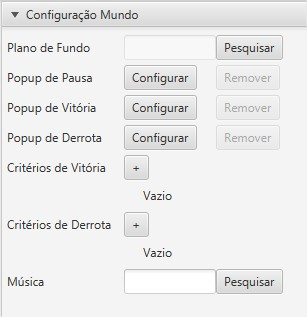
\includegraphics[width=0.4\textwidth]{images/configurar-mundo-1.jpg}
\caption{Painel de configuração de um mundo do jogo na primeira versão da ferramenta.}
\label{fig:configurar-mundo-1}
\end{figure}
\begin{figure}[h]
\centering
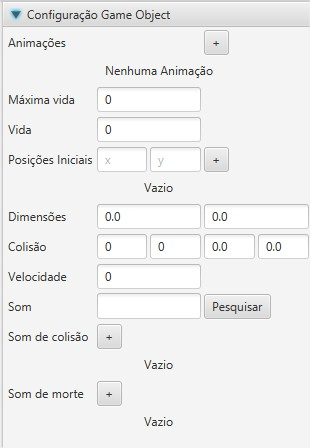
\includegraphics[width=0.4\textwidth]{images/configurar-obj-1.jpg}
\caption{Painel de configuração de um objeto do jogo, existe para os seguintes objetos: ator, inimigo, bônus, opositor e projétil. }
\label{fig:configurar-obj-1}
\end{figure}
\begin{figure}[h]
\centering
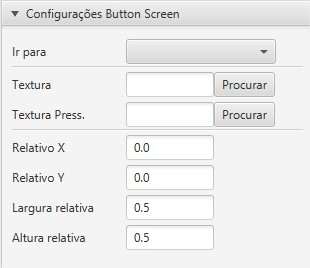
\includegraphics[width=0.4\textwidth]{images/configurar-botao-1.jpg}
\caption{Painel de configuração de um botão na tela do jogo.}
\label{fig:configurar-botao-1}
\end{figure}
\begin{figure}[h]
\centering
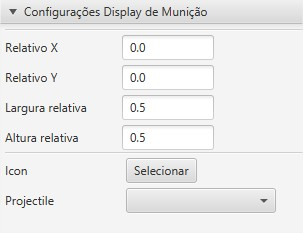
\includegraphics[width=0.4\textwidth]{images/configurar-municao-1.jpg}
\caption{Painel de configuração do mostrador de munição de um projétil do jogo.}
\label{fig:configurar-municao-1}
\end{figure}
\begin{figure}[h]
\centering
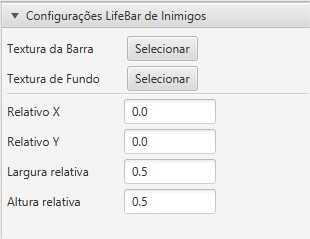
\includegraphics[width=0.4\textwidth]{images/configurar-vida-1.jpg}
\caption{Painel de configuração da barra de vida de um objeto do jogo.}
\label{fig:configurar-vida-1}
\end{figure}

\chapter{Descrição das melhorias} % Joel
\label{chap:melhorias}
Tendo visto os problemas da primeira versão da ferramenta mostrados na secção \ref{chap:problemas}, discuti-se aqui como resolvê-los e o que é necessário para isso. Primeiramente, tem-se uma solução correspondente aos problemas indicados, daí é discutido a sua viabilidade e a implementação técnica. Vale salientar que, os pontos de melhorias mostrados encontram-se implementados na \texttt{ferramenta 2.0}, dessa forma pode ser mostrado o resultado disso (secção \ref{chap:caso}).

\section{Resumo dos pontos de melhoria}
Para cada um dos problemas indicados anteriormente, é necessário determinar a solução de cada um e, além disso, detalhar qual foi o meio técnico. Portanto, tem-se três problemas descritos nas secções \ref{sec:orga-objetos}, \ref{sec:paineis-objetos} e \ref{sec:previa-objetos} e, consequentemente, as respectivas melhorias que estão relacionadas a seguir.

\begin{alineas}
\item \textbf{Organização dos objetos:} Utilizou-se uma árvore que organiza todos os objetos do jogo e deixa claro a relação que existe entre cada um deles. A árvore de objetos possui como raiz o projeto e cada objeto inserido nele é mostrado como seu filho.  Com isso, os botões que representam os itens do jogo na primeira versão da ferramenta foram substituídos por essa árvore.
\item \textbf{Painéis de configuração dos objetos:} Os painéis de configurações permanecem parecidos com a primeira versão da ferramenta, as melhorias visam permitir que as informações alteradas reflitam sempre com a área destinada a simular o jogo, a área de pré visualização, ou seja, no módulo de pré visualização, os painéis terão que interagir para mostrar as mudanças feitas no objeto.
\item \textbf{Pré visualização dos objetos:} A melhoria mais importante desse módulo, consiste em mostrar uma prévia do jogo ao usuário, mostrando os objetos inseridos e configurados, permitindo que o usuário perceba melhor o jogo que ele está criando.
\end{alineas}

\section{A nova tela inicial da ferramenta}
Com o objetivo de implementar as melhorias foi necessário redesenhar a tela inicial da ferramenta, colocando os componentes novos e retirando os que não são mais utilizados. Dessa forma, a árvore de objetos do jogo está localizada a direita da tela, os painéis de configuração dos objetos ficam logo abaixo dela. E, a área de pré visualização é disponibilizada no centro da ferramenta.  A figura \ref{fig:tela_inicial_2} mostra a nova versão da tela inicial e a tabela \ref{table:ferramenta_areas_2} descreve os controles utilizados.

\begin{table}[h]
   \centering
   \begin{tabular}{| l | p{8cm} |}
      \hline
      \textbf{Menu} & Assim como na primeira versão, armazena comandos da ferramenta, a partir do menu pode-se adicionar objetos no jogo, na nova versão da ferramenta o menu substitui a \emph{toolbar} e possui atalhos para facilitar o uso. Por exemplo, \texttt{CTRL + I} para adicionar um inimigo ao jogo. \\
      \hline
      \textbf{Área de pré visualização} & Região  destinada a prévia do jogo, onde os objetos são exibidos da forma mais próxima possível ao jogo. O usuário pode interagir com essa área, selecionando um objeto ou posicionando ele em outro lugar da tela por exemplo.\\
      \hline
      \textbf{Árvore de objetos} & Componente que sumariza todos os objetos existentes no jogo. A árvore é responsável por exibir os objetos em sua hierarquia.\\
      \hline
      \textbf{Painel de configuração} & Painel de configuração do objeto que foi selecionado. Nessa região todas as configurações relacionadas ao objeto selecionado devem ser exibidos \\
      \hline
   \end{tabular}
   \caption{Controles utilizados na segunda versão da ferramenta.}
   \label{table:ferramenta_areas_2}
\end{table}

Os novos controles interagem entre si com o seguinte comportamento, a cada interação na árvore a ferramenta atualiza os painéis e a área de pré visualização de acordo com o objeto que esteja selecionado. Este que, por sua vez, é atualizado também quando algumas propriedades são alteradas no painel. A tabela \ref{table:objetos-atributos} mostra os atributos que quando alterados atualizam a prévia, por exemplo, o campo correspondente ao plano de fundo do mundo (imagem \ref{fig:tela_inicial_2}).

\begin{figure}[h]
\centering
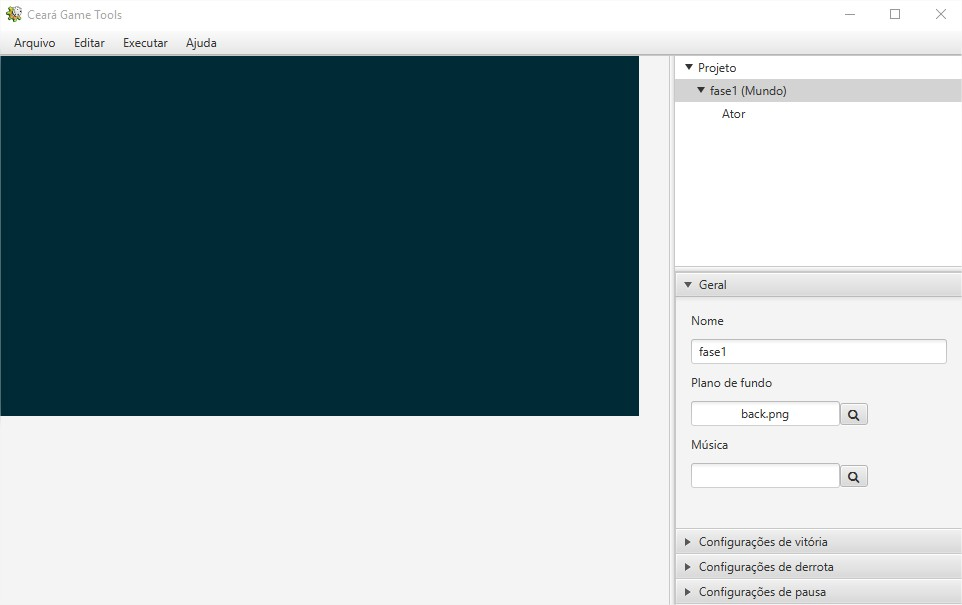
\includegraphics[width=0.8\textwidth]{images/tela_inicial_2.jpg}
\caption{Nova tela inicial da ferramenta com os novos controles que possibilitaram as melhorias.}
\label{fig:tela_inicial_2}
\end{figure}

A seguir, veremos como cada um dos problemas enumerados anteriormente foram resolvidos com base na solução sugerida, além disso como foi a implementação disso.

\section{Descrição técnica}

 A ferramenta é escrita na linguagem \texttt{Java} e utiliza o \emph{framework} \texttt{JavaFX} para a interface do usuário, todo o código escrito para a primeira versão da ferramenta foi reutilizado, incrementando-o a medida que foi preciso na implementação do módulo de \textit{preview}.

Em \emph{JavaFX}, é usado um arquivo XML que descreve o \emph{layout} de uma tela e uma classe que cuida do comportamento dela. Assim, a implementação do módulo de pré visualização, consistiu em alterar esse arquivos XML e suas respectivas classes e, além disso, classes do pacote \texttt{br.ifce.edu.cgt.application.vo}, que receberam objetos customizados que implementam a interface \texttt{DrawbleObject}. A interface \texttt{DrawbleObject} é usada por todos os objetos que são mostrados na área de pré visualização e árvore de objetos, pois define o comportamento que deverá ter os objetos que estarão contidos nessas regiões. Nessa interface, existem dois métodos que são responsáveis por desenhar o objeto e o seu painel de configuração, métodos \texttt{drawObject()} e \texttt{drawConfigurationPanel()} respectivamente.

Com isso é possível visualizar as implementações que foram necessárias para concretizar o objetivo do módulo de pré visualização. O diagrama de classes, mostrando todas as classes que representam esse módulo, pode ser visto nos anexos.

\section{Organização dos objetos}

\subsection{Descrição da solução}
Árvores são ideais para organizar elementos que estão classificados hierarquicamente, com isso, tornou-se a melhor maneira de organizar os objetos da nova versão da ferramenta CGT.
A versão anterior exibia os mundos criados como abas e, dentro de cada uma, os objetos criados eram botões que quando eram clicados exibiam o painel de configuração correspondente ao objeto que foi clicado.
Ao substituir essa visão pela atual, permite-se que, facilmente, o usuário tenha visão de tudo que existe no jogo sem a necessidade de alternar entre abas, vale lembrar que a árvore de objetos ocupa menos espaço na janela, o que permitiu colocar outros controles.
Então, essa melhoria é mais lógica e conveniente, pois agrega mais praticidade a ferramenta.
A imagem \ref{fig:arvore_objetos} mostra um exemplo de uma árvore de objetos para um jogo em criação.

\begin{figure}[h]
\centering
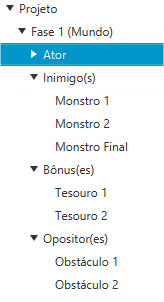
\includegraphics[width=0.2\textwidth]{images/arvore_objetos.png}
\caption{Árvore de objetos da nova versão da ferramenta.}
\label{fig:arvore_objetos}
\end{figure}

\subsection{Implementação técnica}
O objetivo principal da árvore de objetos é garantir que a ferramenta seja atualizada quando um item for selecionado, pois o mesmo deve ser exibido na área de pré visualização e nos painéis de configuração, mas também ela deve organizar os objetos, agrupando-os quando necessário.

Usa-se o objeto \texttt{TreeView} para representar a árvore, onde cada um dos itens é um \texttt{DrawbleObject}. O comportamento que queremos que seja feito, foi implementado com uma fábrica de células customizada que é uma classe que estende de \texttt{TreeCell} e implemente os métodos \texttt{startEdit} e \texttt{updateItem}, chamados quando o usuário interage com a árvore. Nesses métodos, coloca-se a instrução para que seja desenhado os objetos e o painel, ou seja, executa-se os métodos abstratos de \texttt{DrawbleObject} (\texttt{drawObject} e \texttt{drawConfigurationPanel}),  por fim, atribui-se ao \texttt{TreeView} a fábrica customizada assim como é mostrado abaixo (seja \texttt{t} uma instâcia de \texttt{TreeView}):

\begin{lstlisting}[frame=single]
t.setCellFactory(new Callback<TreeView<DrawableObject>,TreeCell<DrawableObject>>(){
    @Override
    public TreeCell<DrawableObject> call(TreeView<DrawableObject> param) {
        return new DrawableObjectTreeCellImpl();
    }
});
\end{lstlisting}

Além do comportamento de redesenhar de acordo com o que foi selecionado na árvore, é importante definir os itens do jogo de acordo com a sua hierarquia, já que a árvore é montada obedecendo isso, a tabela \ref{table:obj-hierarquia} mostra todos os itens e os seus respectivos itens superiores.

\begin{table}[h]
   \centering
   \begin{tabular}{| p{8cm} | l | }
      \hline
      \textbf{Item} & \textbf{Item superior} \\
      \hline
      Projeto & (Raiz) \\
      Mundo & Projeto \\
      Ator, Inimigos, Bônus(es), Opositor(es) & Mundo \\
      Projetil & Ator \\
      Barra de vida & Ator, Inimigo \\
      Munição & Projétil \\
      Tela & Projeto \\
      Botão de tela & Tela \\
      \hline
   \end{tabular}
   \caption{Tabela mostrando a hierarquia que existe entre os objetos de um jogo.}
   \label{table:obj-hierarquia}
\end{table}

Garantir que a ferramenta mostre todos os objetos de acordo com a hierarquia, consiste em adicioná-los corretamente, o \texttt{PreviewPane} faz isso nos métodos que são chamados pelos eventos do menu editar, \texttt{addEnemy} por exemplo.

\section{Painéis de configuração}

Os painéis de configuração na ferramenta são, a grosso modo, os controles responsáveis por receber as informações do usuário e transformá-las em objetos do jogo.
É importante que, os controles usados sejam claros, objetivos e consigam passar para o usuário o significado do que está sendo configurado.

\subsection{Descrição da solução}
Para a implementação do módulo de pré visualização foi necessário aprimorar os painéis existentes na primeira versão da ferramenta, possibilitando as funcionalidades da segunda versão, tem-se a necessidade, por exemplo, de não exibir diálogos de configuração  com tanta frequência, como é feito na versão anterior, pois os mesmos se posicionam na frente da ferramenta  e, consequentemente, da área de pré visualização (ver figura \ref{fig:intro-problema-2} como exemplo de configuração em dialogo).
Além disso, é necessário para os objetos que possuem animação uma prévia dela ou uma forma de selecioná-la melhor no painel de configuração, é o caso do ator e inimigo por exemplo.
Lembrar que, o objetivo é passar para o usuário o que uma determinada configuração representa.

Os painéis são mostrados na ferramenta de forma semelhante aos objetos na pré visualização, ou seja, são disparados através da árvore de objetos, a medida que o usuário seleciona um objeto dela, a configuração correspondente é exibida na região destinada aos painéis.
Em um painel de configuração de um objeto, pode possuir mais de uma configuração para ele, cada configuração deve ser referente a algo e elas são exibidas separadamente.
Usa-se o componente de acordeão para agregar as configurações no painel de acordo com o objetivo dela. Ver a figura \ref{fig:painel_ator} por exemplo, nela temos um painel de configuração de um ator do jogo, percebe-se que cada configuração é separada de acordo com sua finalidade, há uma aba para configurar as animações e outra para configurar as propriedades relacionadas a colisão, por exemplo.

\begin{figure}[h]
\centering
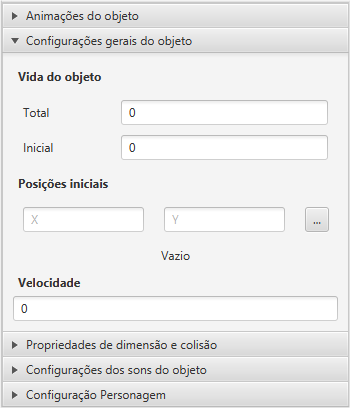
\includegraphics[width=0.4\textwidth]{images/painel_ator.png}
\caption{Painel de configuração de um ator no jogo}
\label{fig:painel_ator}
\end{figure}

\subsection{Implementação técnica}

A implementação dessa melhoria está relacionada a reutilizar os painéis que já existiam e melhorar alguns aspectos, dentre eles, pode-se destacar a configuração das animações do painel responsável por configurar um \emph{game object}.
Na primeira versão da ferramenta, uma animação era adicionada a partir de uma janela \textit{pop up} que mostrava o \textit{sprite} do objeto, então o usuário escolhia dentro de uma matriz o \textit{frame} inicial e final, assim como a finalidade da animação e outras propriedades dela (ver imagem \ref{fig:add_animacao}).
\begin{figure}[h]
\centering
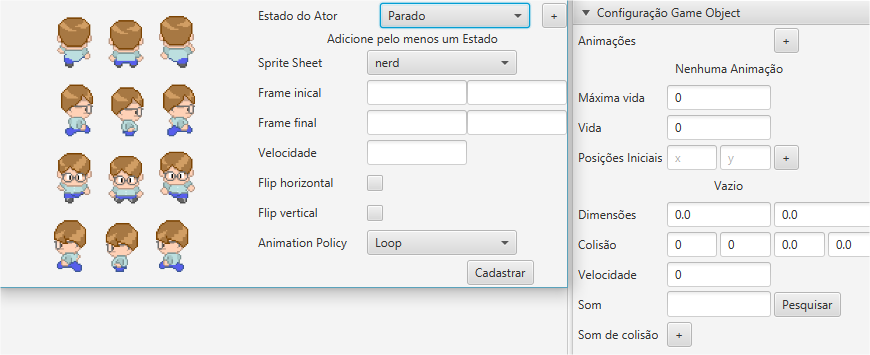
\includegraphics[width=0.8\textwidth]{images/add_animacao_1.png}
\caption{Janela para adicionar animações para um objeto na primeira versão da ferramenta. }
\label{fig:add_animacao}
\end{figure}
Quando há um painel destinado a mostrar as configurações do objeto correspondente, faz-se desnecessário o uso de janela \textit{pop up}, dessa forma, na nova versão da ferramenta as configurações da animação do objeto foram colocadas no painel dele apenas, facilitando a pré visualização e também o manuseio.
Ver imagem \ref{fig:add_animacao_2}, notar que, o que é preciso para configurar uma animação está em três abas desse painel, onde a última aba é uma lista de todas as animações que já existem, a segunda as propriedades da animação e a primeira aba a configuração do quadro inicial e final da animação. Vale notar que o comportamento de selecionar o quadro inicial e final de uma animação para um objeto, tornou-se mais fácil, pois antes  era feito com campos de texto que recebiam as coordenadas $x$ e $y$ do quadro e, na segunda versão, faz-se necessário apenas clicar no quandro que se deseja.
Logo, foi possível transferir tudo para o painel, contribuindo para a coesão da ferramenta e melhorando também no objetivo de pré visualização dos objetos.

De um ponto de vista técnico, os painéis implementados para a nova versão da ferramenta são classes que carregam o arquivo XML que descreve o \textit{layout} (FXML) e, Consequentemente, definem o comportamento.
Além disso, faz-se necessário escrever na função que abre um jogo salvo previamente o comportamento de preencher as informações desses painéis.

\begin{figure}[h]
\centering
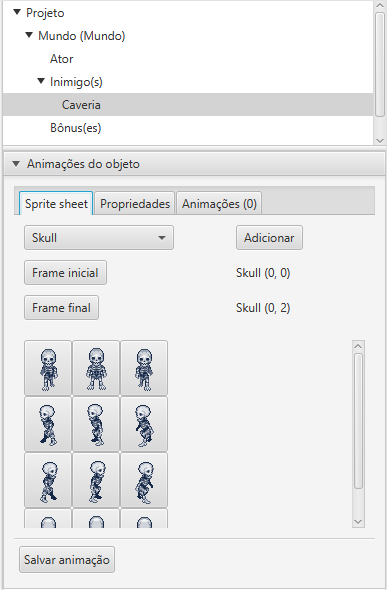
\includegraphics[width=0.5\textwidth]{images/add_animacao_2.png}
\caption{Painel de configuração das animações do objeto na nova versão da ferramenta.}
\label{fig:add_animacao_2}
\end{figure}

\section{Pré visualização}

A pré visualização dos objetos do jogos criados pela ferramenta CGT é a principal melhoria do módulo que foi proposto e desenvolvido com esse trabalho. Vale lembrar que, a nova versão da ferramenta consiste exatamente nos itens presentes neste capitulo, sendo assim, a pré visualização dos objetos é a última funcionalidade que foi implementada e a mais importante, pois como - será visto posteriormente - é a maior responsável por melhorar a experiência do usuário, comparando-a com a versão anterior.

\subsection{Descrição da solução}
Poder conferir o que está sendo produzido, é a principal falta que os usuários da primeira versão da ferramenta sentem. Dessa forma, pode-se dizer que é o maior problema que ela possui. Para resolvê-lo, foi preciso dedicar uma região da janela para uma área de pré visualização do jogo, com isso a ferramenta foi alterada para conter essa área, a árvore de objetos e o painel de configuração (figura \ref{fig:tela_inicial_2}). A área de pré visualização deve conter todos os objetos existentes no jogo para aquele agregador (mundo ou tela do jogo), além disso, o itens devem ser exibidos tais quais seriam no momento de execução do jogo, devem ser fiéis a configuração feita e refletir no resultado real.
Na figura \ref{fig:preview_objetos}, pode-se ver como a tela da ferramenta é usualmente vista pelo usuário, notar que - na área de visualização - é mostrado um mundo em que podem ser vistos dois objetos configurados um ator e um inimigo.

\begin{figure}[h]
\centering
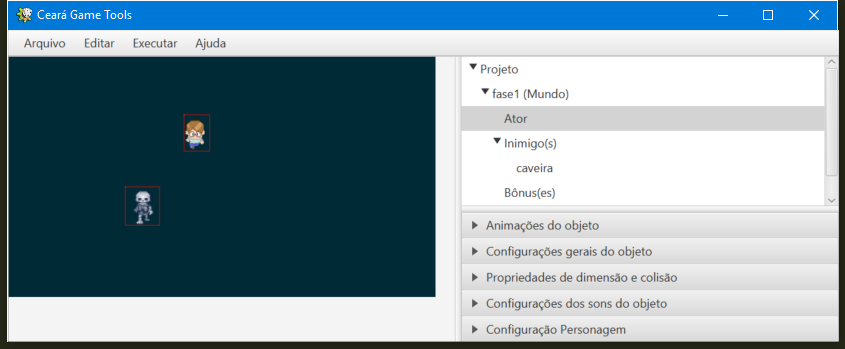
\includegraphics[width=0.8\textwidth]{images/preview1.png}
\caption{Tela da ferramenta mostrando a área de pré visualização com dois objetos configurados.}
\label{fig:preview_objetos}
\end{figure}

\subsection{Implementação técnica}

A construção da pré visualização da ferramenta foi implementada utilizando objetos customizados que possuem três atributos essenciais para o funcionamento dessa funcionalidade:
\begin{alineas}
\item Um atributo que corresponde ao objeto raiz do jogo, por exemplo: ator, inimigo;
\item Um método para desenhar esse objeto raiz na área de pré visualização;
\item Um método para exibir o painel de configuração correspondente ao objeto selecionado;
\end{alineas}

Dessa forma, temos uma interface criada para esse fim, a \texttt{DrawableObject}, a partir daí, foi implementada uma classe abstrata, cujo nome é \texttt{AbstractDrawableObject}, responsável por implementar algumas das tarefas comuns de todos esses objetos desenháveis.
Com isso, pode-se ainda estender essa classe abstrata e gerar classes especificas aos objetos que necessitam de uma prévia, então foram criadas classes com o sufixo \texttt{Drawable}, por exemplo \texttt{CGTGameActorDrawable} que tem o objetivo de descrever cada uma das propriedades citadas anteriormente.

Então, por definição, um objeto desenhável deve prover de meios para representar um objeto raiz do projeto, que são os objetos que estão no pacote \texttt{cgt.core} dentro do módulo \texttt{core} do projeto (ver tabela \ref{table:modulos}). Os meios que um desenhável possui são os métodos \texttt{drawObject} e \texttt{drawConfigurationPanel} que são responsáveis por exibir o objeto e o painel de configuração respectivamente.
Esses objetos desenháveis, são criados pelo usuário e inseridos na árvore de objetos (assim como explicado na secção \ref{sec:orga-objetos}), no momento de inserção, o método que os desenha é chamado e, então, a pré visualização é exibida.
A medida que, o usuário vai configurando esses objetos no respectivo painel de configuração, a prévia dele é atualizada na área de visualização.
Isso é possível, graças a criação de métodos do tipo \emph{callback} que existem em todos os painéis de configuração que necessitam que as mudanças sejam exibidas assim que feitas, notar que, esse método é chamado pelo próprio painel toda vez que algum atributo relevante é modificado, por exemplo, a dimensão e posição de um objeto, assim como é mostrado na figura \ref{fig:obj_preview_tamanho}.

\begin{figure}[h]
\centering
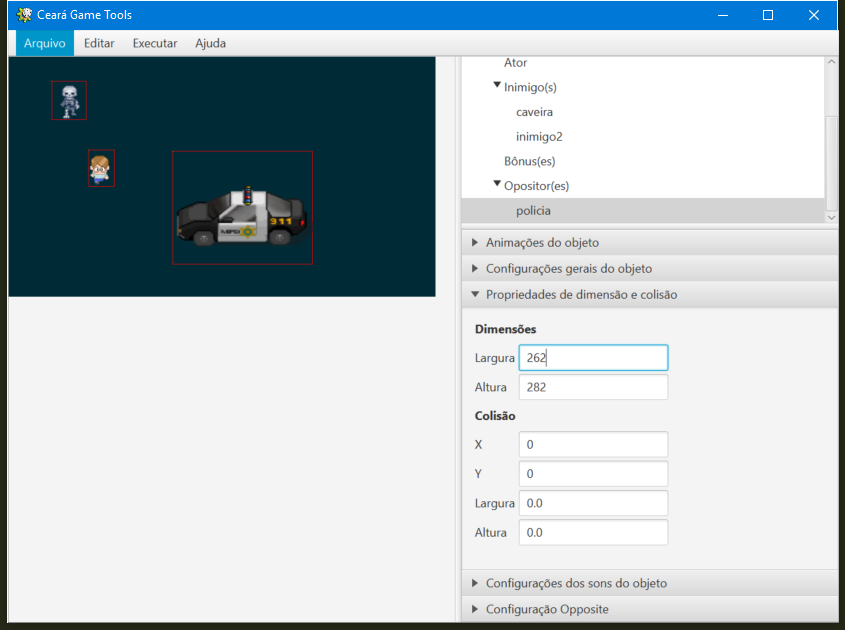
\includegraphics[width=0.8\textwidth]{images/preview2.png}
\caption{Exemplo de dimensão do objeto sendo percebida no momento que é alterada na configuração}
\label{fig:obj_preview_tamanho}
\end{figure}

Ou seja, toda vez que é detectado um evento de mudança no campo de texto do tamanho do objeto, o método de \textit{callback} - que é um objeto Java da classe \texttt{Runnable}, mas no painel é um atributo cujo nome é \texttt{onUpdateRunnable} - é executado da forma é mostrado a seguir. Notar que, quem cria o objeto que corresponde ao painel de configuração é que deve determinar o conteúdo desse método \texttt{callback}, dessa forma, é garantido que o painel seja compatível com a ferramenta.

\begin{mylisting}[h]
\begin{lstlisting}
boundsH.focusedProperty().addListener(new ChangeListener<Boolean>() {
 @Override
 public void changed(ObservableValue<? extends Boolean> observable,
   Boolean oldValue, Boolean newValue) {
      if (!newValue) {
         /** comportamento para mudar a altura do objeto */
      }

      if (onUpdateRunnable != null) {
         onUpdateRunnable.run();
      }
   }});
\end{lstlisting}
\end{mylisting}


\chapter{Estudo de caso}
\label{chap:caso}
\section{Análise dos resultados}
\section{Comparativo}
\section{Jogo exemplo}
\section{Projeto de extensão}

\chapter{Conclusão e trabalhos futuros}
\label{chap:conclcsao}

\postextual
\bibliography{references}


\begin{anexosenv}
   \partanexos
   \chapter{Manual da ferramenta}

   Após as melhorias implementadas na nova versão da ferramenta, foi preciso atualizar o manual existente em trabalhos anteriores \cite{monografia:aquino}. Usou-se a mesma estrutura do manual anterior, atualizando-o para adequar-se às novas telas implementadas.
   Então, com este novo manual será possível encontrar uma descrição sucinta da ferramenta CGT(Ceará Game Tools), mostrando todas as suas funcionalidades e imagens que explicam as suas configurações.
   Dividido em duas partes, a primeira parte deste manual é referente a configuração de um jogo usando a ferramenta, já a segunda parte se refere a explicação de cada funcionalidade que o CGT possui.
   Assim, o usuário possuirá um exemplo prático e a parte teórica caso já saiba o que deseja.

   \section{Configuração de um jogo com a ferramenta}
   Com o intuito de mostrar as funcionalidades que a ferramenta possui, será demonstrada a criação de um jogo com a ferramenta CGT.

   \subsection{Criar tela}
   Uma tela representa uma tela do jogo inicial, podendo ser encontrada como uma tela de configurações, uma tela de créditos, entre outros exemplos.
   Para criar uma tela basta ir no menu: \texttt{Editar$\rightarrow$Adicionar$\rightarrow$Tela} da ferramenta, ou o atalho: \texttt{ALT+T} (ver figura \ref{fig:add_tela}).
   No painel de configuração de uma tela, o usuário pode configurar o plano de fundo e o áudio.
   No exemplo a seguir foi selecionada uma imagem para o plano de fundo e adicionado botões a ela, figura \ref{fig:add_tela_2}.

   Agora serão configurados os botões que foram adicionados a tela.
   Como o procedimento é o mesmo para todos os botões, será demonstrada apenas a configuração de um. Nele serão configurados ação, imagem, posicionamento e dimensão do botão.
   A ação do botão, representado pelo “ir para”, será selecionada outra tela previamente criada ou um mundo, que será explicado ao longo do texto.
   Quanto a imagem do botão, será selecionada uma para quando se encontrar no estado normal e outra para quando for pressionado, causando a ideia de efeito ao clicar sobre o botão.
   O seu posicionamento na tela e dimensão são configurados com base na tela e os valores devem variar de 0 a 1, representando a porcentagem da tela. A área de pré-visualização permite arrastar o botão para a posição desejada, atualizando o painel de configuração em seguida (figura \ref{fig:add_botao}).
   Com isso, a ferramenta permite ao usuário criar telas de acordo com a necessidade do jogo e com os botões que lhe forem preciso.

   \begin{figure}[h]
   \centering
   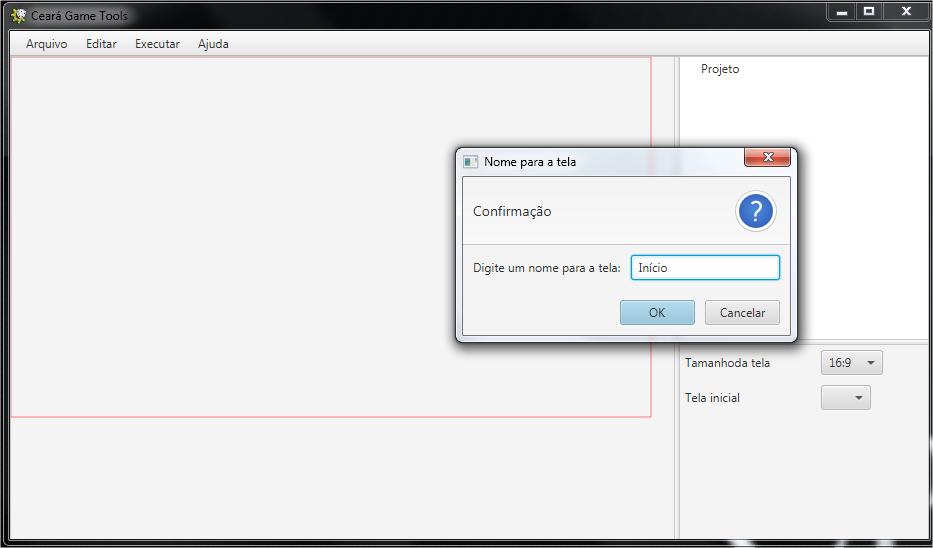
\includegraphics[width=0.7\textwidth]{images/add_tela.png}
   \caption{Inserindo uma nova tela na ferramenta.}
   \label{fig:add_tela}
   \end{figure}

   \begin{figure}[h]
   \centering
   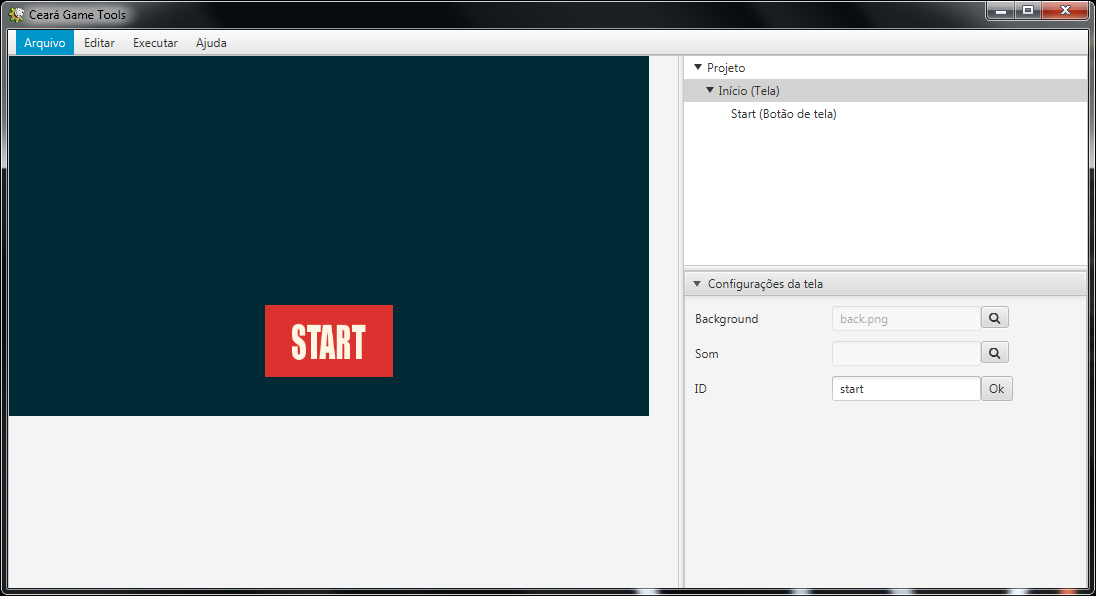
\includegraphics[width=0.7\textwidth]{images/add_tela_2.png}
   \caption{Tela de um jogo exemplo sendo configurada.}
   \label{fig:add_tela_2}
   \end{figure}

   \begin{figure}[h]
   \centering
   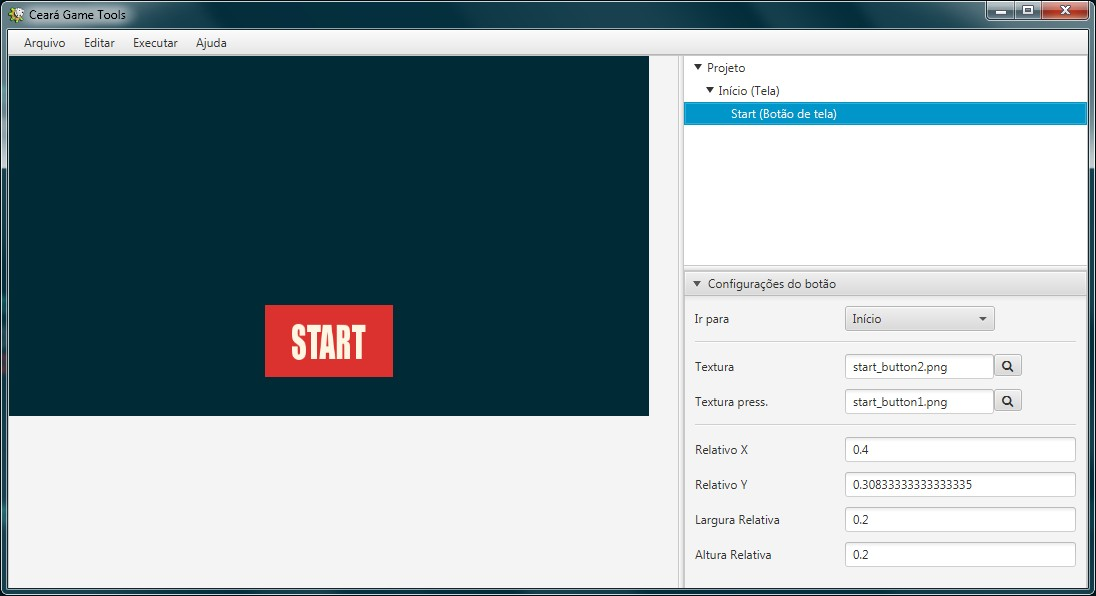
\includegraphics[width=0.7\textwidth]{images/add_botao.jpg}
   \caption{Configurando um botão em tela de exemplo do jogo.}
   \label{fig:add_botao}
   \end{figure}

   \subsection{Criar mundo}
   O botão de uma tela pode levar a um mundo. Um mundo pode ser o seu jogo ou uma fase dele e é constituído de vários objetos que serão configurados mais adiante.
   Para criar um mundo basta ir no menu: \texttt{Editar$\rightarrow$Adicionar$\rightarrow$Mundo} da ferramenta, ou o atalho: \texttt{ALT+M} (ver figura \ref{fig:add_mundo}).
   Como mostrado na imagem \ref{fig:add_mundo_2}, o mundo possui algumas características gerais, que são: nome, plano de fundo e música.
   Na figura \ref{fig:add_mundo_3}, temos as configurações do critério de vitória para esse mundo que podem ser cinco (eliminar inimigos, sobreviver, pegar bônus, completar percurso e atingir pontuação) e da mensagem que será exibida quando o jogador vencer.
   Na figura \ref{fig:add_mundo_4}, temos as configurações de derrota desse mundo, os critérios podem ser: ator morrer ou contagem regressiva, uma mensagem de derrota também pode ser configurada.
   Além dessas mensagens de derreta e vitória, na figura \ref{fig:add_mundo_5}, é possível configurar a mensagem que será exibida quando o mundo estiver em pausa.
   Por fim, na figura \ref{fig:add_mundo_6}, tem-se o painel de configuração da câmera do mundo.

   \begin{figure}[htb]
   \centering
   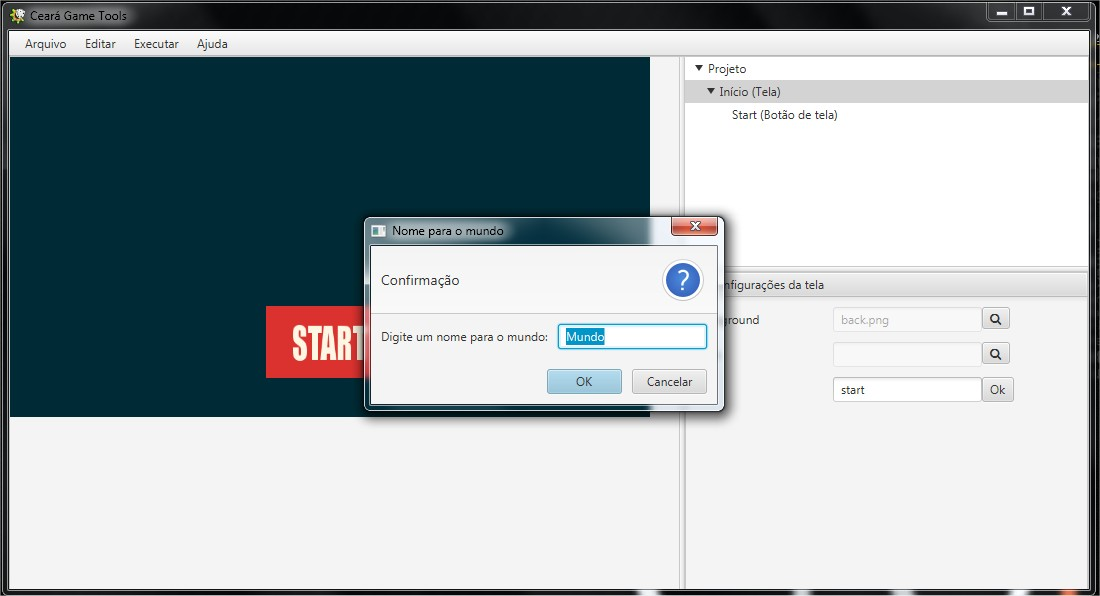
\includegraphics[width=0.7\textwidth]{images/add_mundo.jpg}
   \caption{Adicionando um mundo na nova versão da ferramenta}
   \label{fig:add_mundo}
   \end{figure}
   \begin{figure}[htb]
   \centering
   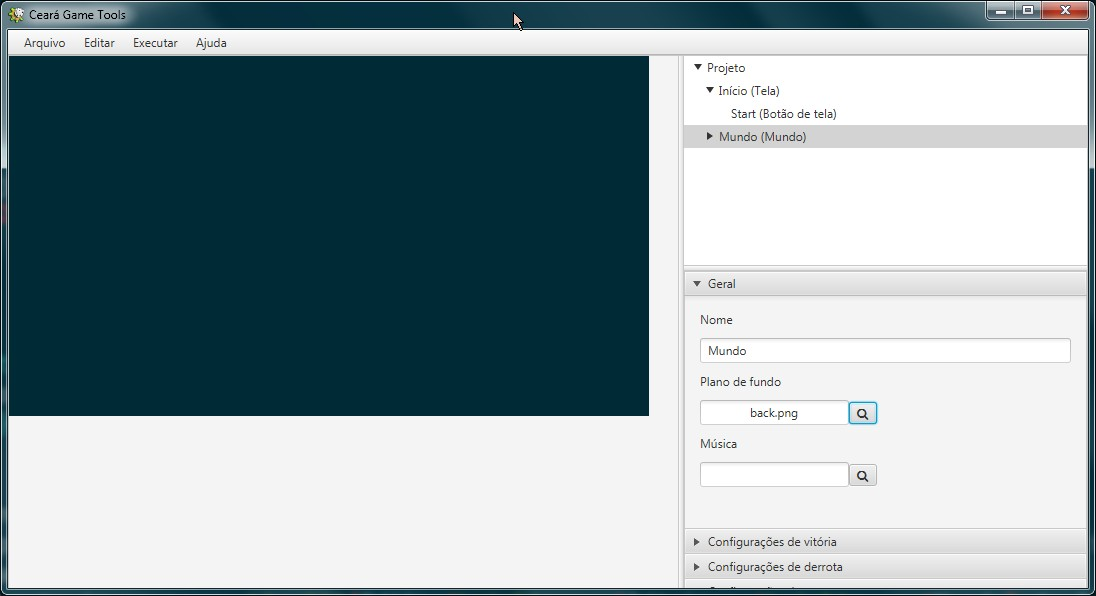
\includegraphics[width=0.7\textwidth]{images/add_mundo_2.jpg}
   \caption{Propriedades gerais de um mundo.}
   \label{fig:add_mundo_2}
   \end{figure}
   \begin{figure}[htb]
   \centering
   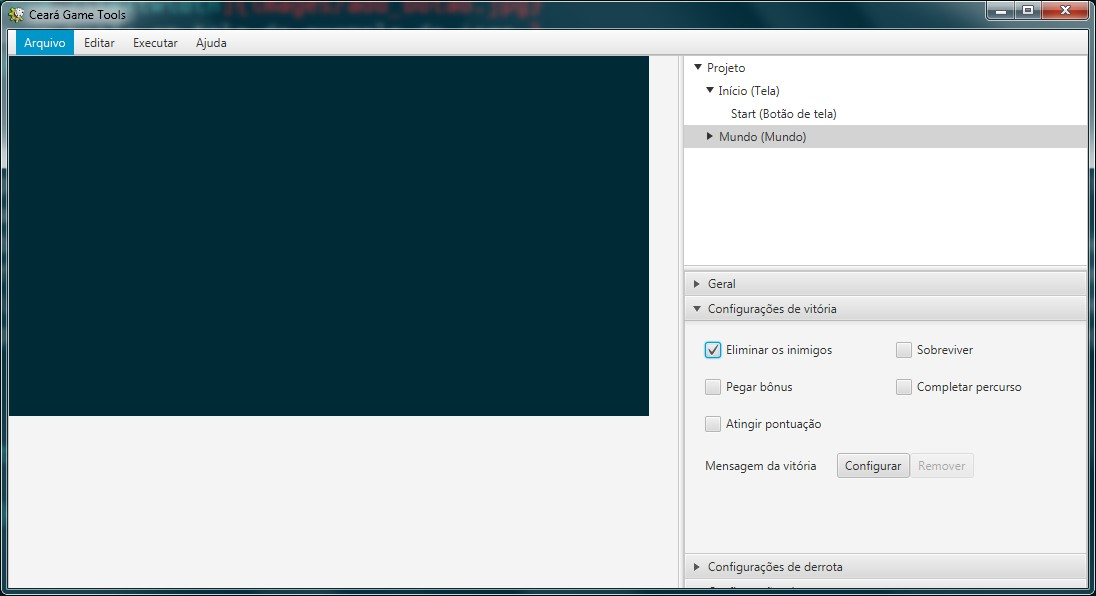
\includegraphics[width=0.7\textwidth]{images/add_mundo_3.jpg}
   \caption{Propriedades de vitória do mundo.}
   \label{fig:add_mundo_3}
   \end{figure}
   \begin{figure}[htb]
   \centering
   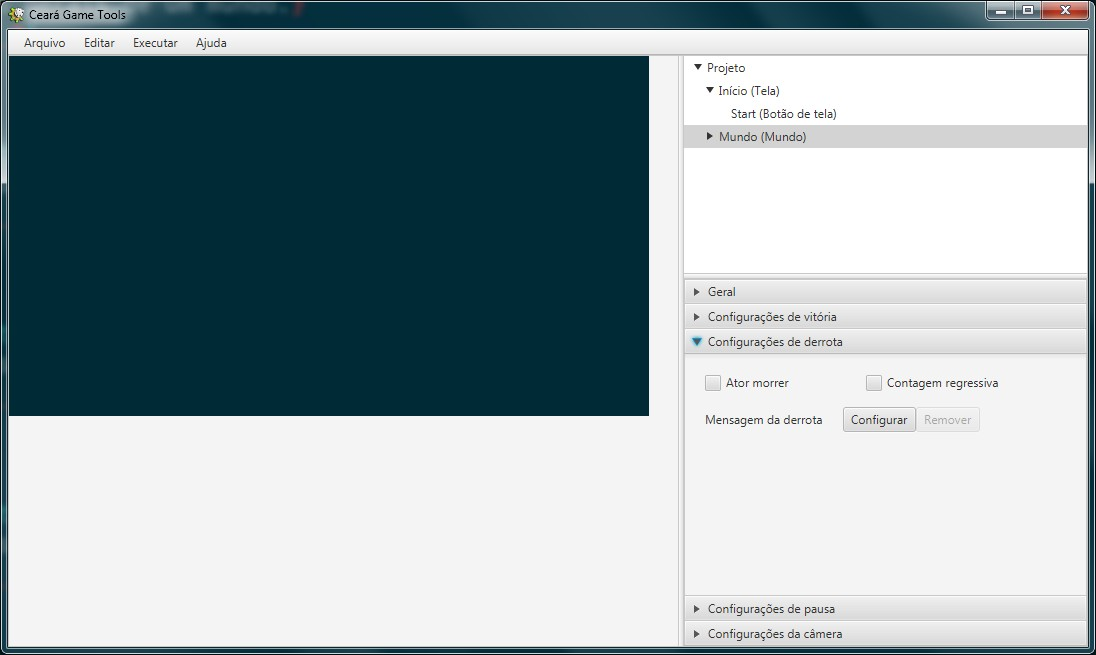
\includegraphics[width=0.7\textwidth]{images/add_mundo_4.jpg}
   \caption{Propriedades de derrota do mundo.}
   \label{fig:add_mundo_4}
   \end{figure}
   \begin{figure}[htb]
   \centering
   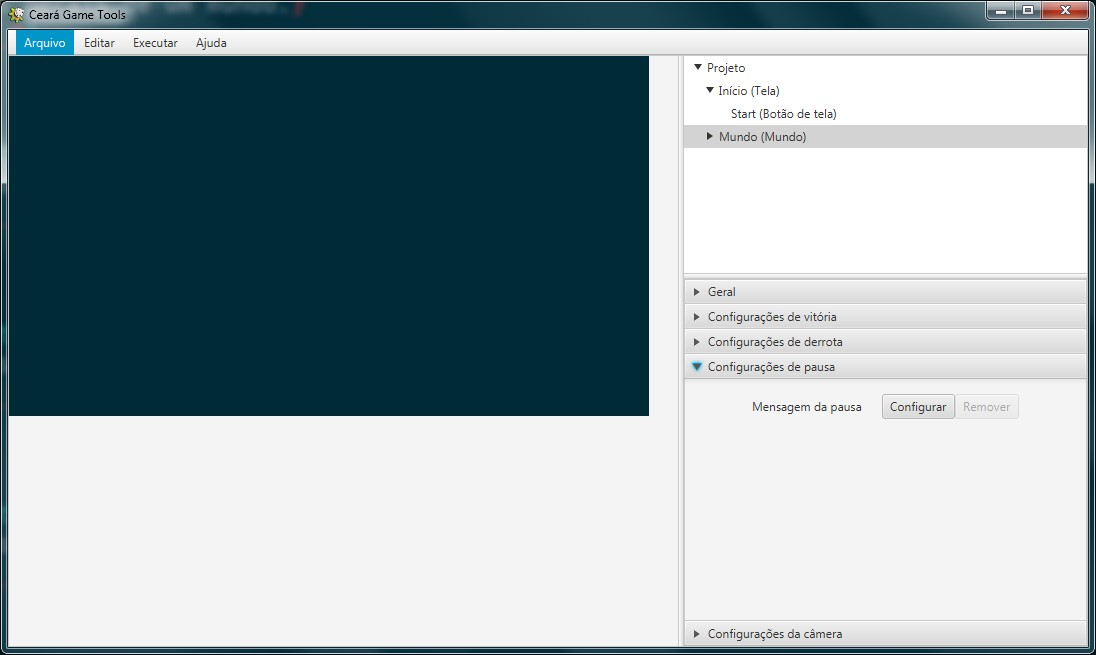
\includegraphics[width=0.7\textwidth]{images/add_mundo_5.jpg}
   \caption{Propriedades da pausa do mundo.}
   \label{fig:add_mundo_5}
   \end{figure}
   \begin{figure}[htb]
   \centering
   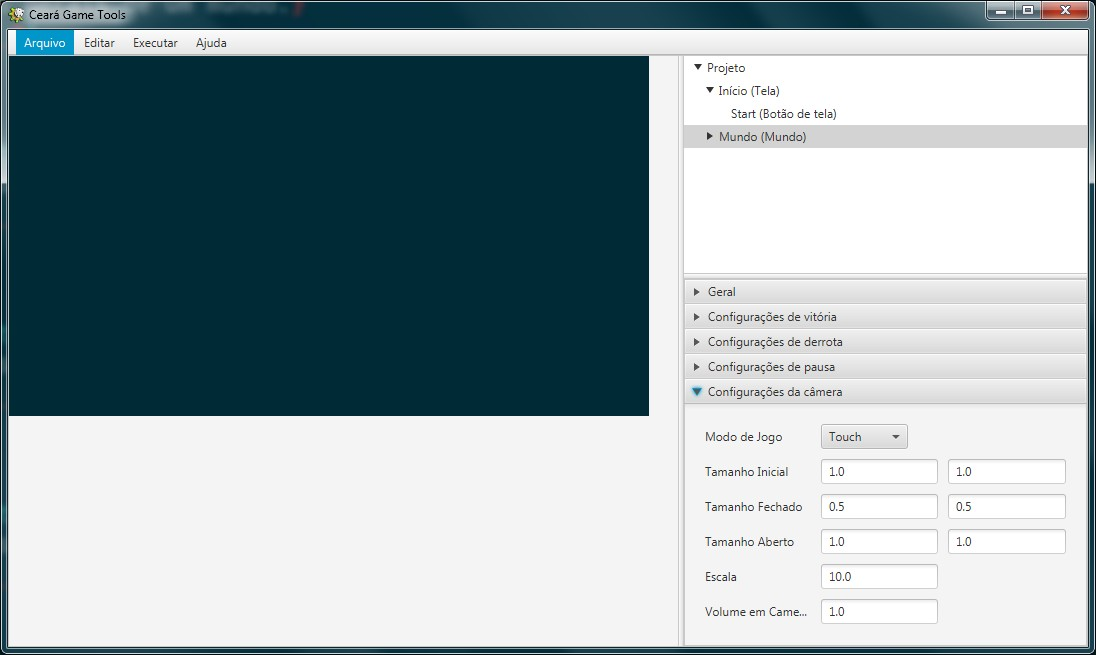
\includegraphics[width=0.7\textwidth]{images/add_mundo_6.jpg}
   \caption{Propriedades da câmera do mundo.}
   \label{fig:add_mundo_6}
   \end{figure}

   \subsubsection{Configurar mensagens}
   A configuração das mensagens são todas iguais, então será demonstrada apenas a configuração um deles. Para configurar será necessário ajustar posicionamento, dimensão, imagens e botões. Uma mensagem deve possuir três imagens bases, que precisam ser do tipo PNG, são elas o fundo, a borda horizontal e a borda do canto inferior. A imagem de fundo será o plano de fundo, as imagens de borda horizontal e canto inferior direito são imagens usadas para se definir a borda de toda a janela da mensagem. Ver figura \ref{fig:config_msg}.

   \begin{figure}[h]
   \centering
   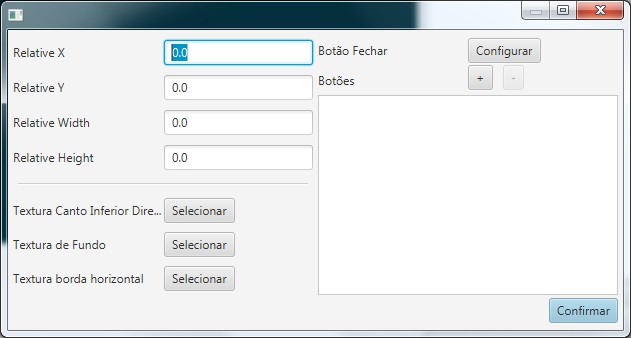
\includegraphics[width=0.8\textwidth]{images/config_msg.jpg}
   \caption{Janela de configuração de uma mensagem no mundo, seja ela para vitória, derrota ou pausa.}
   \label{fig:config_msg}
   \end{figure}

   \subsubsection{Ator principal}


   \subsubsection{Configurar opositores}


   \subsubsection{Configurar inimigos}


   \subsubsection{Bônus}


   \subsubsection{Configurar projétil}


   \subsubsection{Configurar HUD}


   \section{Telas da ferramenta}


   \subsection{Configurar tela}


   \subsection{Configurar mundo}


   \subsubsection{Configurações gerais}


   \subsubsection{Configurar \emph{pop-up}}


   \subsubsection{Configurar critérios de vitória}


   \subsubsection{Critérios de derrota}


   \subsubsection{Configurar \emph{spritesheet}}


   \subsubsection{Configurar animação (ator, inimigo, opositor, bônus, projétil)}


   \subsubsection{Configuração comum dos objetos(ator, inimigo, opositor, bonus,projétil)}


   \subsection{Configurações específicas do ator}


   \subsubsection{Configurações das ações do ator}


   \subsection{Configurações especificas dos inimigos}


   \subsubsection{Comportamento sino}


   \subsubsection{Comportamento \emph{fade}}


   \subsubsection{Comportamento onda}


   \subsection{Configurações específicas dos opositores}


   \subsection{Configurações específicas dos bônus}


   \subsection{Configurar projétil}


   \subsubsection{Configuração do posicionamento}


   \subsection{Configurar \emph{HUDs}}


   \subsubsection{Configuração do tela de munição}


   \subsubsection{Configuração do barra de vida dos inimigos}


   \subsubsection{Configuração barra de vida objeto}


   \section{Executar projeto}


   \section{Configurar game}


   \section{Exportar projeto}


   \section{Gerar chave de assinatura}

teste

   \chapter{Diagramas de classes}
   \label{chap:diagramas}
   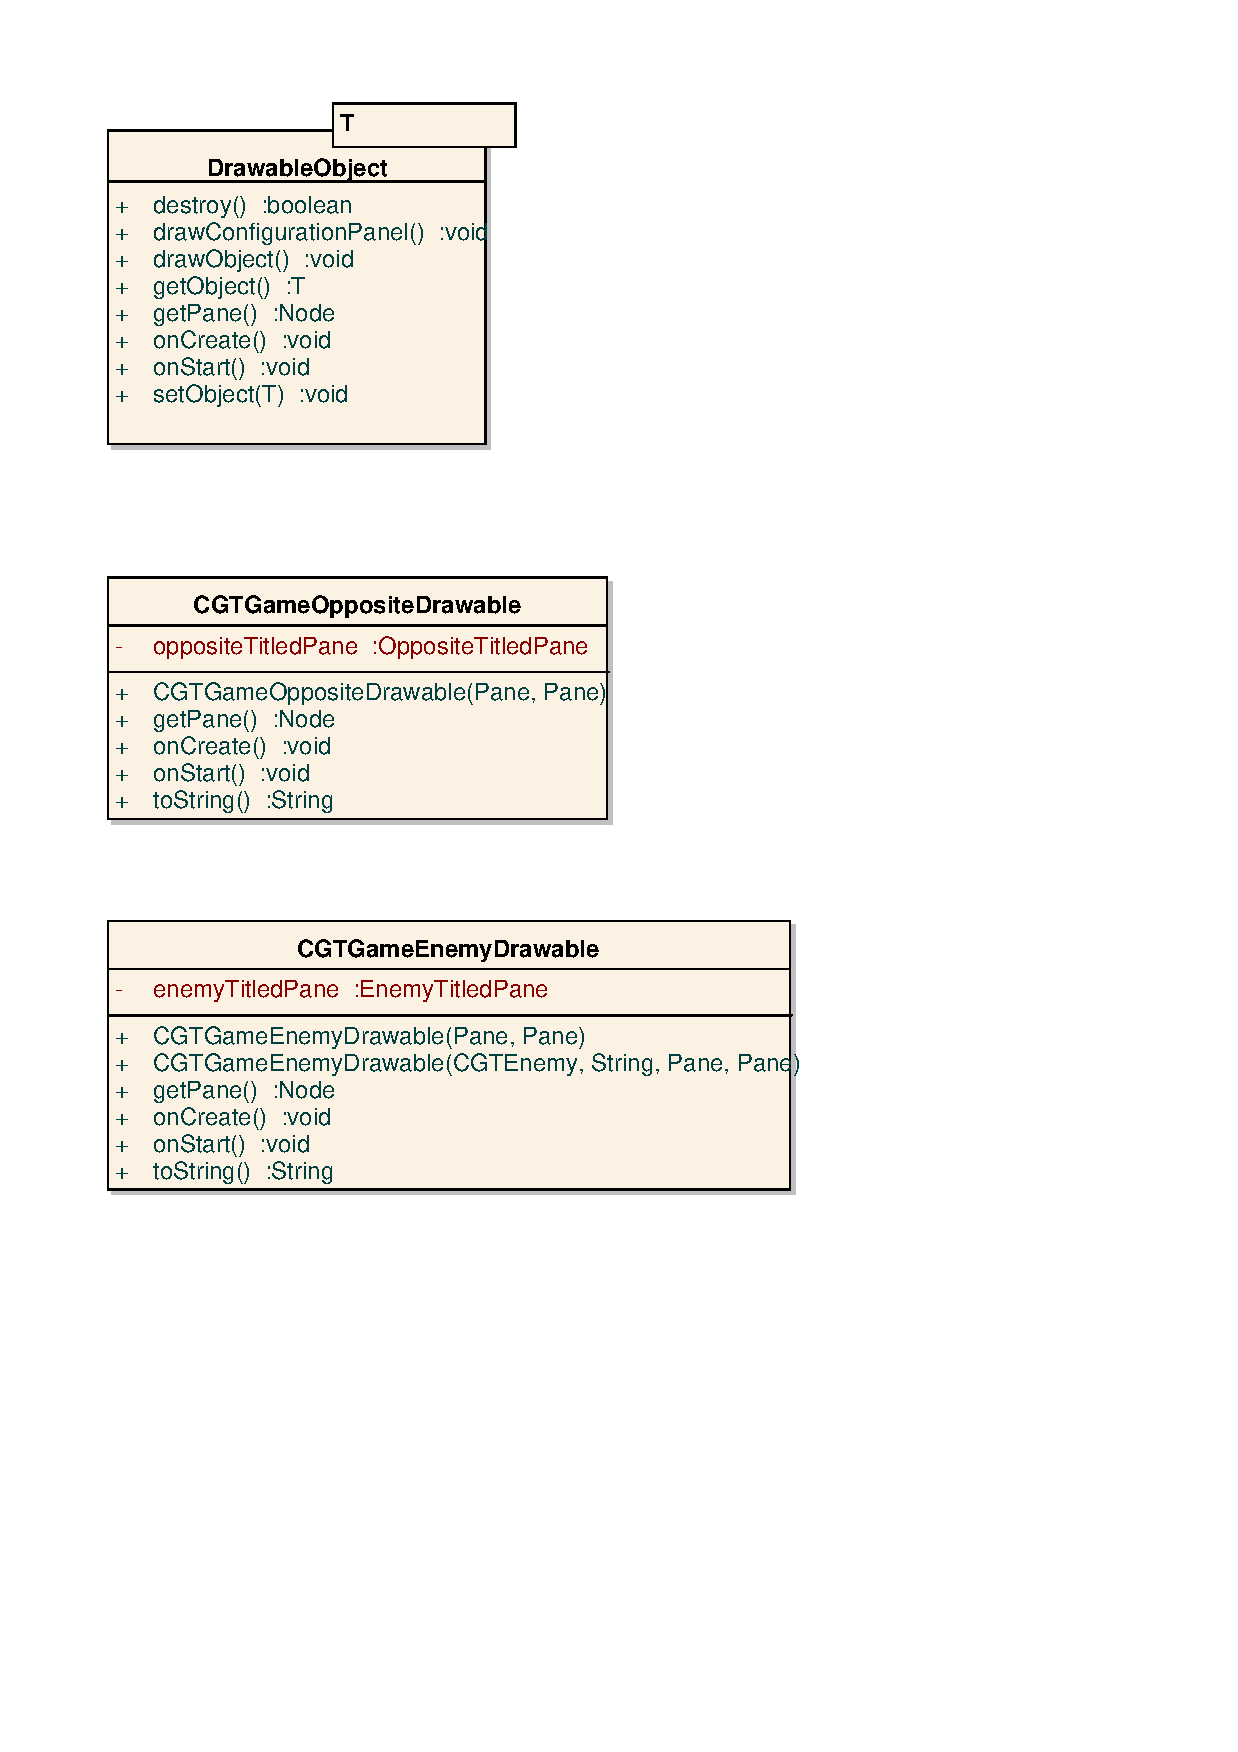
\includepdf[pages=-]{ClassModel.pdf}
\end{anexosenv}
\phantompart
\printindex
\end{document}
